\documentclass{article}
\usepackage[a4paper,left=1in, right=1in, top=1in, bottom=1in]{geometry}
\usepackage{subcaption}
\usepackage{graphicx}
\usepackage{color}
\usepackage{listings}
\DeclareGraphicsExtensions{.pdf,.png,.jpg}
\graphicspath{ {./images/} }
\definecolor{mygreen}{rgb}{0,0.6,0}
\definecolor{mygray}{rgb}{0.5,0.5,0.5}
\definecolor{mymauve}{rgb}{0.58,0,0.82}
\lstset{commentstyle=\color{mygreen},language=c}

\begin{document}
\title{Gibbot v4 Code}
\author{Andrew Griesemer}
\maketitle
\section{I\textsuperscript{2}C}
The Gibbot PCB uses I\textsuperscript{2}C communication between the dsPIC in each link. The dsPICs also each communicate with a MPU-9150 Nine Axis Sensor via I\textsuperscript{2}C. To maintain compatibility, the I\textsuperscript{2}C protocol between the two dsPICs will be based off of the I\textsuperscript{2}C used by the MPU-9150. For communication between the two dsPICs the dsPIC in the top link will act as master and the dsPIC in the lower link will act as slave. For communication between the dsPICs and the MPU-9150 both dsPICs will act as master. This section references three documents in the footnotes. Those documents are:
\begin{description}
\item{MPU-9150 Product Specification Revision 4.3}

http://www.invensense.com/mems/gyro/documents/PS-MPU-9150A-00v4\_3.pdf
\item{dsPIC33/PIC24 Family Reference Manual: Inter-Integrated Circuit (I2C) Section}

http://ww1.microchip.com/downloads/en/DeviceDoc/70000195f.pdf
\item{dsPIC33EPXXX(GP/MC/MU)806/810/814 Data Sheet (10/17/2012)}

http://ww1.microchip.com/downloads/en/DeviceDoc/70616g.pdf
\end{description}

\subsection{Commands}
\begin{figure}[h!]
	\centering
	\begin{subfigure}{0.5\textwidth}
		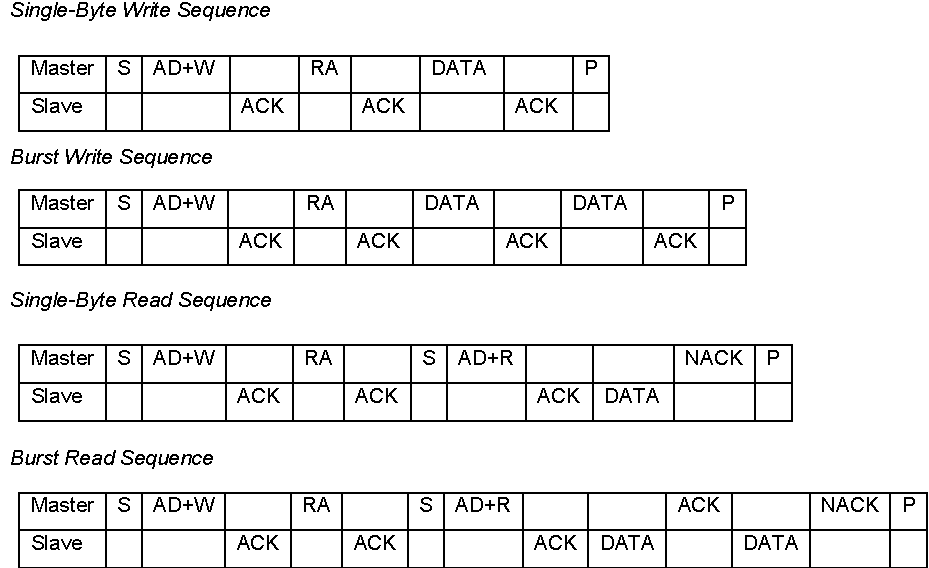
\includegraphics[width=\textwidth, page=1]{i2c}
	\end{subfigure}
	\quad
	\begin{subfigure}{0.4\textwidth}
		\includegraphics[width=\textwidth, page=2]{i2c}
	\end{subfigure}
	\caption{I\textsuperscript{2}C commands for MPU-9150\protect\footnotemark}
	\label{i2c}
\end{figure}
\footnotetext{From MPU-9150 Product Spec p 34-35}
The module is responsbible for the four different commands shown in Figure \ref{i2c}. 

\subsection{Slave Configuration}
Because the slave dsPIC does not control the timing of the I\textsuperscript{2}C messages communication is handled by the the I\textsuperscript{2}C Slave Interrupt. The initialization code for the I\textsuperscript{2}C does four things:
\begin{enumerate}
\item{Sets a 7 bit address that the I\textsuperscript{2}C module will recognize as the device address.}
\item{Configures a global pointer variable RegPtr to point to the address of the first slot in an array RegBuffer.}
\item{Initialize the I\textsuperscript{2}C slave interrupt}
\item{Turn on the I\textsuperscript{2}C module}
\end{enumerate}

\begin{lstlisting}[xleftmargin=\parindent,frame=L]
void initialize_I2C_Slave(void){
    I2C2ADD = 0b1101101;    //Sets the 7 bit slave address
    RegPtr = &RegBuffer[0]; //Reg pointer points to beginning of RegBuffer
    IFS3bits.SI2C2IF = 0;   //Clear interrupt flag
    IPC12bits.SI2C2IP = 7;  //Set priority to 6
    IEC3bits.SI2C2IE = 1;   //Enable I2C 2 Slave interrupt

    I2C2CONbits.I2CEN = 1;  //Enable I2C 2
}
\end{lstlisting}

At the beginning of a transmission the I\textsuperscript{2}C module detects the start condition and compares the following address byte with the I2C2ADD register. If the address matches, the I\textsuperscript{2}C Slave Interrupt flag is set, the D/A bit in the I2C2STAT register is cleared and the R/W bit in the I2C2STAT register is modified to reflect the R/W bit in the command. If the address does not match, the module takes no action and all following bytes are ignored until after a stop condition is detected.

 

\begin{lstlisting}[xleftmargin=\parindent,frame=L]
void __attribute__((interrupt, no_auto_psv)) _SI2C2Interrupt(void) {
    /* I2C module will read to detect the address 11011010 being sent by the
     * master. The final bit of the address is the Read/Write
     * bit which is interpreted by the module.
     *   1101101R
     */
    int i;
    unsigned char tempvar = 0;
    if(I2C2STATbits.R_W){      //If Master device is sending a write command
        if(!I2C2STATbits.D_A){ //If byte received was device address
            tempvar = I2C2RCV; //Dummy read to clear RCV register
            nextByteData = 0;
            nextByteAddr = 1;  //The following byte will be the register address
        } else {               //If byte received was data
            if(nextByteAddr){  //If last byte recieved was device address this
                               //byte is the address of the register to be read.
                RegPtr = RegPtr + I2C2RCV; //Set pointer to desired register
                nextByteAddr = 0;
                nextByteData = 1;     //The following byte will be data
            } else if(nextByteData){  //If last byte recieved was register
                                      //address this byte is data to be written
                *RegPtr = (unsigned char)I2C2RCV; //write data to register
                RegPtr = RegPtr + 1;  //Increment pointer by 1 for burst write
            }
        }
    } else {                   //If Master device is sending a read command
        encoder_Read(MOTENC);
        I2C2TRN = *RegPtr;     //Load the transmit register with data
        
        __delay32(12); //Delay for at least 100ns (4 clock cycles)
                       //minimum number of delay cycles for delay32 is 12.
        I2C2CONbits.SCLREL = 1;//Release the clock stretch
        //Wait for the transmit buffer to clear or for a timeout.
        while(I2C2STATbits.TBF && (i < 4000000)){
            i++;
        }
        if(i >= 4000000){ //If timeout indicate with LED and restart I2C module
           LED3 = 0;
           I2C2CONbits.I2CEN = 0;
           I2C2CONbits.I2CEN = 1;
        }
    }
    IFS3bits.SI2C2IF = 0;
}
\end{lstlisting}

\end{document}